% Contactless-to-Contact Fingerprint Recognition with CMRA
% LaTeX source for Overleaf
% Biometric Security Course Project - NIT Warangal

\documentclass[12pt,a4paper]{article}
\usepackage[utf8]{inputenc}
\usepackage[T1]{fontenc}
\usepackage{lmodern}
\usepackage[margin=1in]{geometry}
\usepackage{amsmath,amssymb,amsfonts}
\usepackage{graphicx}
\usepackage{booktabs}
\usepackage{array}
\usepackage{multirow}
\usepackage{caption}
\usepackage{float}
\usepackage{hyperref}
\usepackage{enumitem}
\usepackage{titlesec}

\hypersetup{
    colorlinks=true,
    linkcolor=blue,
    filecolor=magenta,
    urlcolor=cyan,
    pdftitle={Contactless-to-Contact Fingerprint Recognition with CMRA},
    pdfauthor={Aryan Desai, Naman Sinha, Saurabh Bharrdwaj, Sayan Das}
}

\titleformat{\section}{\Large\bfseries}{\thesection}{1em}{}
\titleformat{\subsection}{\large\bfseries}{\thesubsection}{1em}{}

\renewcommand{\arraystretch}{1.15}

\begin{document}

% ===================== TITLE PAGE =====================
\begin{titlepage}
\centering
\vspace*{2cm}
{\LARGE\textbf{National Institute of Technology Warangal}\par}
\vspace{0.5cm}
{\large Biometric Security --- Course Project\par}
\vspace{3cm}
{\Huge\textbf{Contactless-to-Contact Fingerprint Recognition}\par}
\vspace{1cm}
{\Large Cross-Modal Relational Alignment (CMRA)\par}
\vspace{0.5cm}
{\large with Risk-Controlled Abstention\par}
\vfill
\vspace{1cm}
{\large A reproducible study on the HKPolyU Contactless 2D to Contact-based 2D database\par}
\vspace{1cm}
{\large Team:\par}
Aryan Desai \textbullet\ Naman Sinha \textbullet\ Saurabh Bharrdwaj \textbullet\ Sayan Das\par
\vspace{1cm}
{\large November 2026\par}
\vfill
\end{titlepage}

% ===================== ABSTRACT =====================
\section*{Abstract}
\addcontentsline{toc}{section}{Abstract}

Contactless fingerprint acquisition is hygienic and portable, but matching a contactless finger photo against a conventional contact-based print remains difficult because the two modalities differ in illumination, perspective, ridge scale, distortion and noise. Contactless-to-contact verification is essential for remote onboarding and access control, yet most published methods are evaluated mainly on contactless-to-contactless data. VerifNet-style systems use pairwise contrastive training and fixed fusion weights, while transformer-based methods require external training data and GPU resources, leaving a gap for lightweight reproducible cross-modal matchers. We overcome these limitations with Cross-Modal Relational Alignment (CMRA), a single embedding trained to preserve cross-modal relational identity structure using identity-balanced PK batches, ArcFace supervision, prototype consistency and relational consistency losses. CMRA comprises four modules: a fixed scattering front-end for CPU-efficient feature extraction, an ArcFace-trained embedding network, a prototype consistency loss aligning cross-modal identity centres, and a relational consistency loss matching cross-modal similarity structure. Extensive experiments on HKPolyU CL2CB under a controlled identity-disjoint split show CMRA achieves 16.80\% EER and 29.55\% TAR@FAR=1\%, surpassing the reproduced VerifNet-style baseline (36.11\% EER), the fixed DL+MM fusion (32.83\% EER) and the ISE-only baseline (19.56\% EER). These results show that cross-modal relational alignment, not score fusion alone, is the key contribution for lightweight contactless-to-contact fingerprint verification.

\vspace{0.3cm}
\textbf{Keywords:} contactless fingerprint; cross-modal matching; relational alignment; ArcFace; CMRA; HKPolyU.

% ===================== TABLE OF CONTENTS =====================
\newpage
\tableofcontents
\newpage

% ===================== 1. INTRODUCTION =====================
\section{Introduction}

Fingerprint recognition is one of the most widely deployed biometric modalities, but conventional systems require physical contact with a sensor, raising hygiene concerns and leaving latent prints. Contactless acquisition using a smartphone camera avoids these issues but creates a new problem: matching a contactless finger photo against a legacy contact-based print is difficult because the two modalities differ in illumination, perspective, ridge scale, distortion and noise. Existing methods such as VerifNet combine scattering-wavelet features, contrastive Siamese networks and minutiae matching with fixed fusion, but they are evaluated mainly on contactless-to-contactless data and use pairwise rather than identity-level supervision. Transformer-based methods achieve lower error but require external training data, large backbones and GPU resources, making them impractical for CPU-only deployment. In this work, we propose Cross-Modal Relational Alignment (CMRA), which trains a single embedding to preserve cross-modal relational identity structure using identity-balanced batches and consistency losses, eliminating score fusion as the main contribution.

\textbf{Key contributions:}
\begin{itemize}[leftmargin=*]
    \item A new cross-modal relational alignment training objective for fingerprint matching that preserves cross-modal relational identity structure.
    \item Removal of the VerifNet-style Siamese branch from the proposed system, replacing it with a single embedding and eliminating score fusion as the main contribution.
    \item Risk-controlled abstention for reliable verification at low false-accept rates, allowing the system to abstain on low-confidence comparisons.
\end{itemize}

The report is organised as follows: Section 2 reviews related work, Section 3 describes the CMRA methodology, Section 4 presents experiments and results, and Section 5 concludes with future work directions.

% ===================== 2. RELATED WORK =====================
\section{Related Work}

\textbf{Traditional methods:} Lin and Kumar pioneered contactless-to-contact fingerprint matching on HKPolyU using hand-crafted ridge-based features and COTS matchers. Their Multi-Siamese and RTPS+DCM approaches achieved strong results but rely on classical image processing rather than learned representations.

\textbf{CNN-based methods:} VerifNet combines fixed scattering-wavelet features, a contrastive Siamese network and minutiae matching with a fixed 90/10 score fusion. While compact and CPU-efficient, its pairwise training and fixed fusion weight limit its adaptation to the harder contactless-to-contact setting.

\textbf{Transformer methods:} Ridgeformer uses a vision transformer with cross-attention and multi-stage contrastive training to achieve 2.83\% EER on HKPolyU. This strong performance requires training on four external datasets and GPU resources, limiting its reproducibility.

\textbf{Attention-based CNNs:} MANet uses a minutiae map to guide attention in a deep learning branch for contactless fingerprint recognition. Its attention mechanism is evaluated mainly on contactless-to-contactless matching, not cross-modal verification.

\textbf{Systematic review:} Kaplesh et al. provide a systematic review of end-to-end contactless fingerprint recognition frameworks, identifying preprocessing, domain shift and matching as key bottlenecks. As a survey, it does not propose a new matching method but highlights the need for reproducible benchmarks.

% ===================== 3. METHODOLOGY =====================
\section{Methodology}

\subsection{Overview}
Figure~\ref{fig:pipeline} shows the CMRA pipeline. Both images are preprocessed and passed through a fixed scattering front-end. The resulting features are fed to a single embedding network trained with ArcFace on identity-balanced PK batches containing both contactless and contact impressions of the same finger. Two consistency losses are added: prototype consistency aligns the mean embedding of each identity across the two modalities, and relational consistency matches the cross-modal similarity (Gram) structure so that the two modalities agree on who is close to whom. At inference, embeddings are compared with cosine similarity. The VerifNet-style Siamese branch and score fusion are removed from the proposed system; they appear only as baselines. Risk-controlled abstention optionally rejects low-confidence comparisons.

\begin{figure}[H]
    \centering
    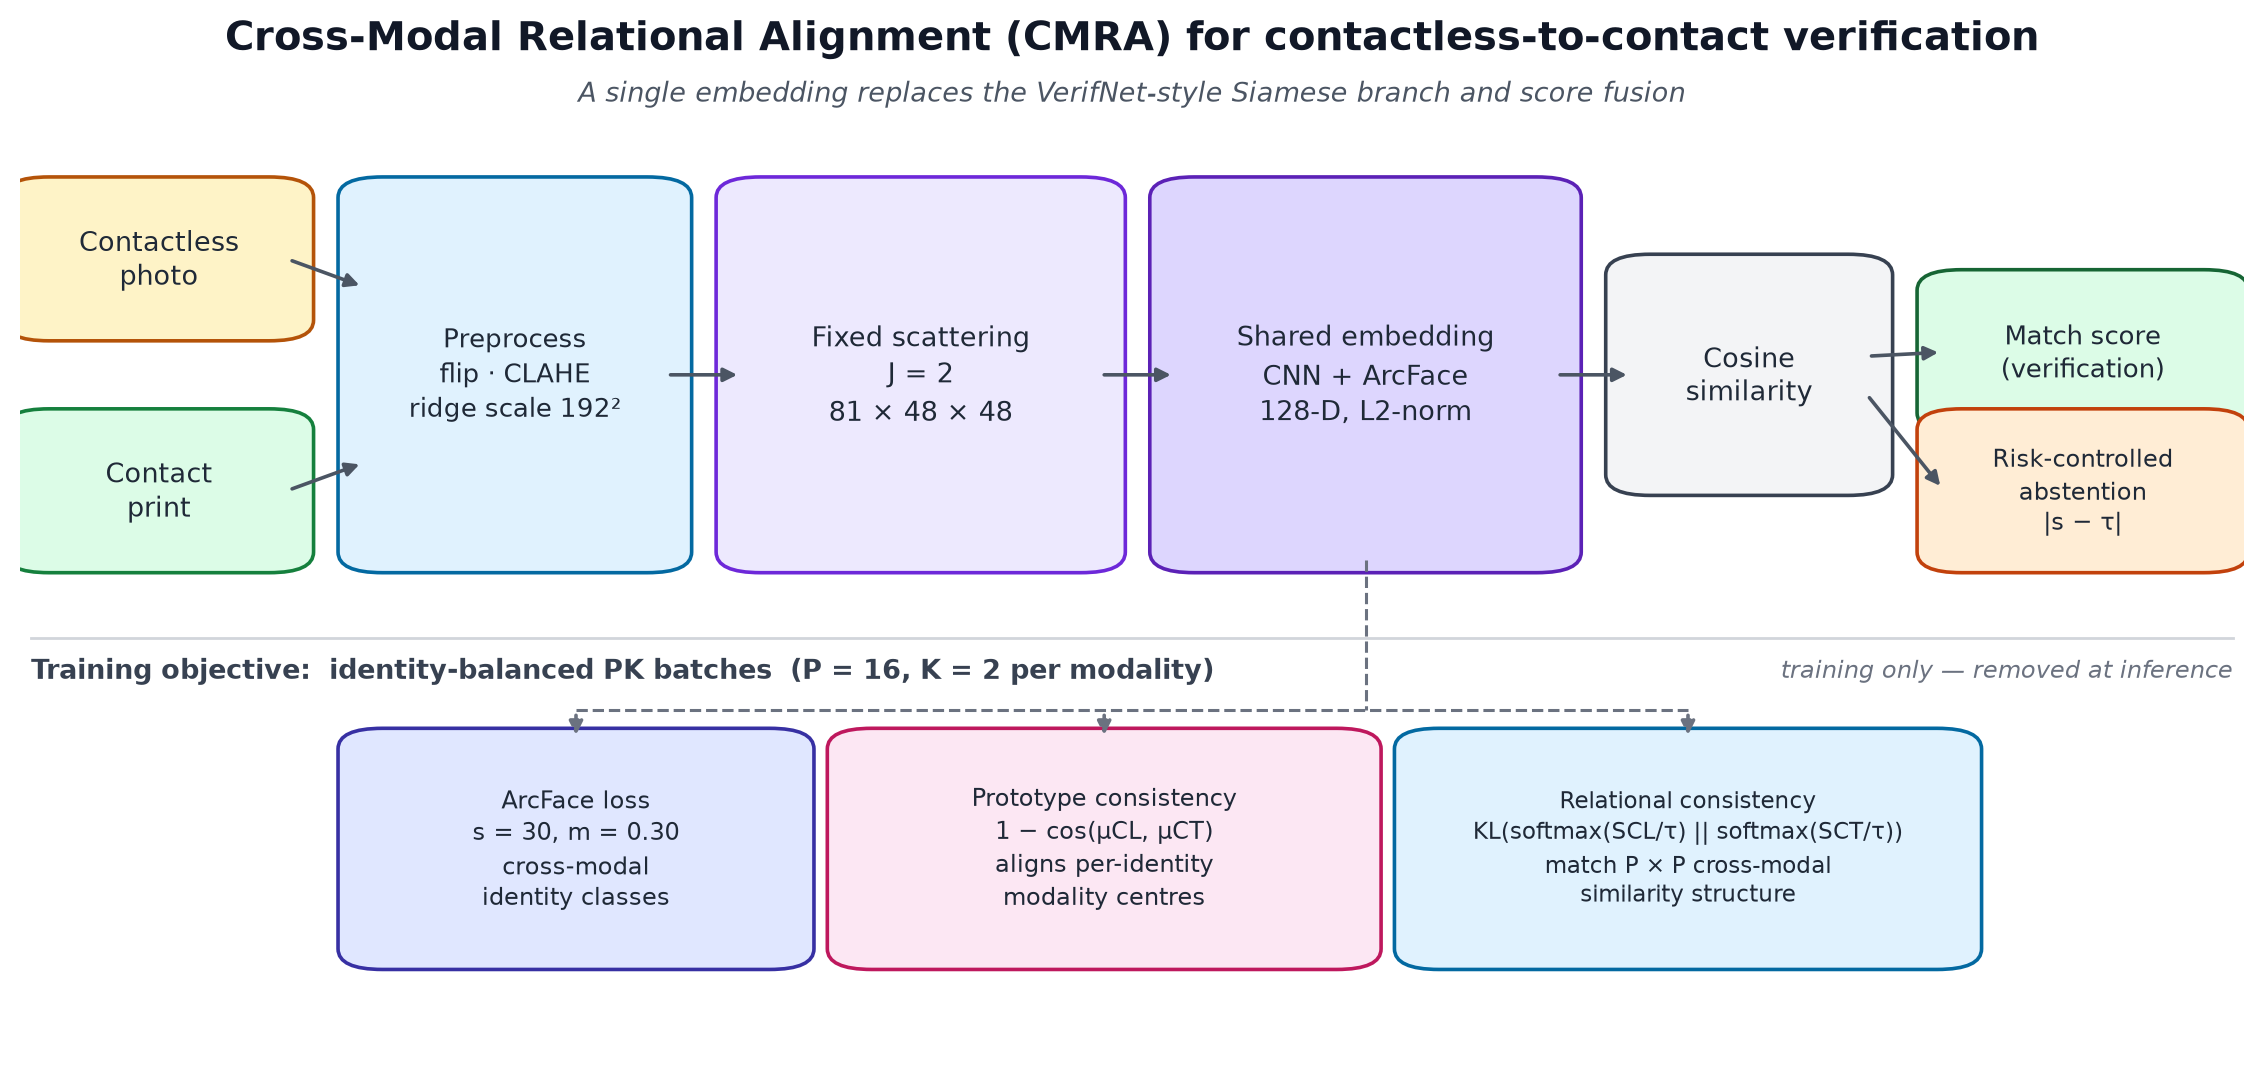
\includegraphics[width=0.7\textwidth]{pipeline.png}
    \caption{CMRA pipeline: scattering front-end, identity-balanced PK batches, ArcFace, prototype consistency and relational consistency losses.}
    \label{fig:pipeline}
\end{figure}

\subsection{Scattering Front-End}
Each preprocessed image is encoded with a fixed 2D scattering transform (Kymatio, J=2) producing 81 channels of size 48$\times$48. Scattering features preserve texture and ridge-frequency information without learning early-layer filters, making them cheap to compute and memory-map on a CPU-only machine.

\subsection{Identity-Balanced PK Batches}
Instead of random image batches or random pairs, each training batch contains $P$ identities with $K$ contactless and $K$ contact impressions per identity ($P\times 2K$ images total). Both modalities of the same finger share one class label, so the network is trained directly on the cross-modal identity structure.

\subsection{Training Objective}
The embedding $f$ is trained with ArcFace loss: for embedding $e_i$ and class weight $w_y$, the logit of the correct class is $s \cdot \cos(\theta_y + m)$, where $\theta_y$ is the angle between $e_i$ and $w_y$, with scale $s=30$ and margin $m=0.30$. Two consistency losses are added.

\textbf{Prototype consistency:} $\mu_i^{\text{cl}}$ and $\mu_i^{\text{ct}}$ are the L2-normalised mean embeddings of identity $i$ in the contactless and contact sets. The loss is $\mathcal{L}_{\text{proto}} = \text{mean}_i (1 - \cos(\mu_i^{\text{cl}}, \mu_i^{\text{ct}}))$, pulling the two modality centres together.

\textbf{Relational consistency:} $S^{\text{cl}}$ and $S^{\text{ct}}$ are the $P\times P$ cosine-similarity matrices of the contactless and contact prototypes. The loss is the symmetric KL divergence between softmax($S^{\text{cl}}/\tau$) and softmax($S^{\text{ct}}/\tau$), forcing the two modalities to agree on the relative layout of identities without forcing absolute coordinates to coincide.

The full objective is $\mathcal{L} = \mathcal{L}_{\text{arcface}} + \lambda_1\mathcal{L}_{\text{proto}} + \lambda_2\mathcal{L}_{\text{rel}}$. Four ablations are run: ArcFace only, ArcFace + prototype, ArcFace + relational, and ArcFace + both (full CMRA).

\subsection{Inference and Abstention}
At inference, two images are embedded and compared with cosine similarity. Risk-controlled abstention ranks comparisons by confidence $|\text{score} - \tau|$ and optionally rejects low-confidence pairs, trading coverage for lower error rate.

% ===================== 4. EXPERIMENT AND RESULTS =====================
\section{Experiment and Results}

\subsection{Setup Used}
All experiments run on an Intel Core Ultra 9 285H laptop with 16 CPU threads and 32 GB RAM, without a discrete GPU. PyTorch 2.14.1 (CPU build), Kymatio 0.3.0, scikit-learn 1.9.1, OpenCV 5.0 and NumPy 2.2 are used. The embedding network (0.13M parameters) trains for 30 epochs in about 15 minutes with AdamW (lr=$10^{-3}$, weight decay=$10^{-4}$), cosine learning-rate decay, batch size 64 ($P=16$ identities, $K=2$ images per modality), and gradient clipping at 1.0. Checkpoint selection uses the lowest validation EER.

\begin{table}[H]
    \centering
    \caption{Implementation settings.}
    \label{tab:settings}
    \begin{tabular}{ll}
    \toprule
    Component & Setting \\
    \midrule
    Scattering transform & Kymatio 2D, J=2, 81$\times$48$\times$48 \\
    Embedding & 128-D, CNN body + linear projection \\
    ArcFace & scale 30, margin 0.30, label smoothing 0.05 \\
    Optimiser & AdamW, lr 1e-3, weight decay 1e-4, cosine schedule \\
    Training & 30 epochs, PK batches ($P$=16, $K$=2), $\pm$2-cell translation \\
    Checkpoint selection & lowest validation EER (no TTA) \\
    Inference & 5-view shift TTA, cosine similarity \\
    Bootstrap & 500 identity-cluster resamples \\
    \bottomrule
    \end{tabular}
\end{table}

\begin{figure}[H]
    \centering
    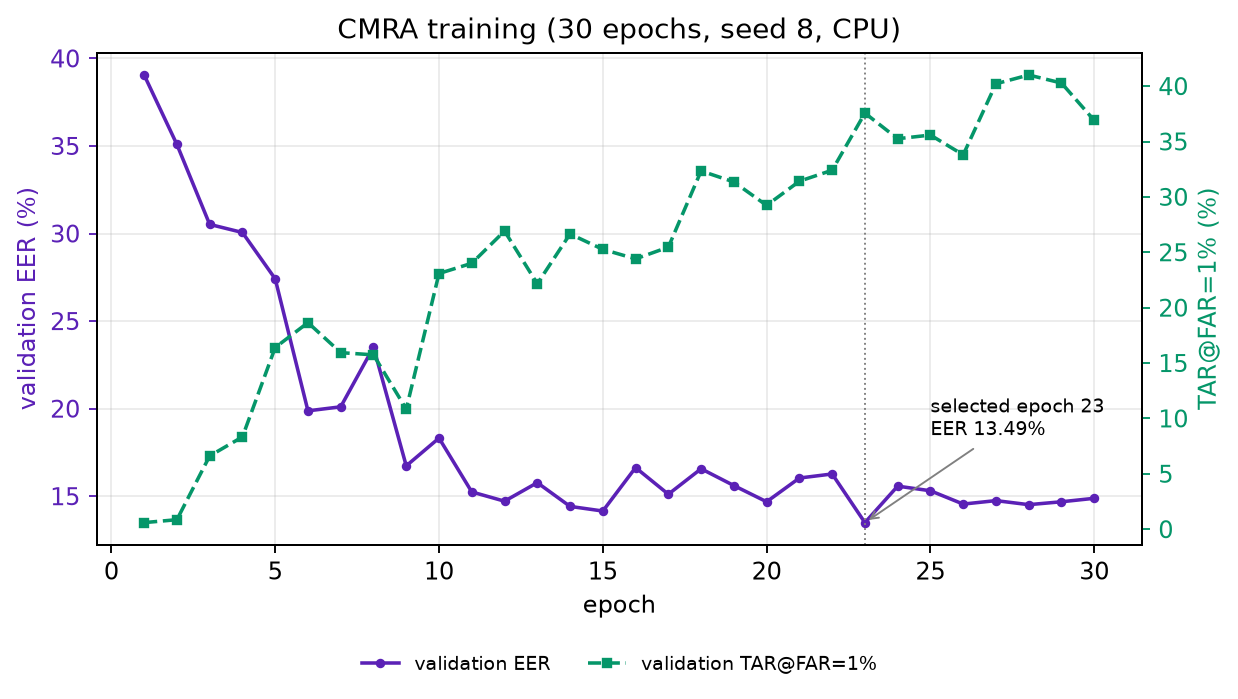
\includegraphics[width=0.62\textwidth]{training_curve.png}
    \caption{CMRA training curve (seed 8): validation EER and TAR@FAR=1\% per epoch; the selected checkpoint is epoch 23.}
    \label{fig:training}
\end{figure}

\subsection{Benchmark Dataset}
Experiments use the Hong Kong Polytechnic University (HKPolyU) Contactless 2D to Contact-based 2D Fingerprint Images Database. It contains 336 fingers, 2,976 contactless and 2,976 contact images (5,952 total), with six impressions per finger per session. A subset of 160 fingers was acquired in a second session. The controlled protocol uses an identity-disjoint split: 201 training, 34 validation and 101 test identities, with no identity overlap across splits. The primary test set has 10,728 balanced pairs (5,364 genuine, 5,364 impostor). A supplementary cross-session study uses 48 test identities present in both sessions, with 3,456 genuine and 3,456 impostor cross-session pairs.

\begin{table}[H]
    \centering
    \caption{HKPolyU CL2CB dataset and protocol summary.}
    \label{tab:dataset}
    \begin{tabular}{ll}
    \toprule
    Property & Value \\
    \midrule
    Fingers / identities & 336 \\
    Images & 2,976 contactless + 2,976 contact (5,952 total) \\
    Sessions & First: 336 fingers; second: 160 fingers \\
    Train / validation / test & 201 / 34 / 101 identities (disjoint) \\
    Primary test pairs & 10,728 (5,364 genuine, 5,364 impostor) \\
    Cross-session test & 48 identities, 3,456 genuine + 3,456 impostor \\
    \bottomrule
    \end{tabular}
\end{table}

\subsection{Performance Metrics}
Verification performance is summarised by the equal error rate (EER), the true accept rate at false accept rates of 1\% and 0.1\% (TAR@FAR=1\%, TAR@FAR=0.1\%), and ROC/DET curves. Confidence intervals use an identity-cluster bootstrap (500 resamples of test identities). Risk-controlled abstention is evaluated with error-vs-coverage curves and area under the risk-coverage curve (AURC).

\subsection{Results}
Table~\ref{tab:ablation} shows the ablation of CMRA components on the 10,728-pair test set. ArcFace-only training on identity-balanced PK batches already reaches 19.41\% EER, improving on the ISE-only v1 baseline at 19.56\%. Adding prototype consistency (18.23\%) and relational consistency (17.74\%) each help, and full CMRA reaches 16.80\% EER with 29.55\% TAR@FAR=1\% and 7.20\% TAR@FAR=0.1\%. The relational term alone beats prototype alone at this seed, showing that matching cross-modal similarity structure is the strongest single addition.

\begin{table}[H]
    \centering
    \caption{CMRA ablation results (percentages, seed 7). CI is an identity-cluster bootstrap.}
    \label{tab:ablation}
    \begin{tabular}{lcccc}
    \toprule
    Method & Test EER & TAR@1\% & TAR@0.1\% & 95\% CI \\
    \midrule
    ISE (v1 baseline) & 19.56 & 28.24 & 4.05 & [17.3, 21.7] \\
    CMRA arc-only (PK batches) & 19.41 & 24.33 & 4.34 & [17.5, 21.3] \\
    CMRA + prototype & 18.23 & 27.44 & 5.87 & [15.8, 20.6] \\
    CMRA + relational & 17.74 & 28.93 & 6.99 & [15.5, 20.1] \\
    CMRA full (prototype + relational) & 16.80 & 29.55 & 7.20 & [14.7, 19.3] \\
    \bottomrule
    \end{tabular}
\end{table}

Table~\ref{tab:v1compare} compares full CMRA against the v1 pipeline on the same test set. CMRA seed 7 reaches 16.80\% EER, beating the v1 best fusion (quality-aware LR) at 18.16\% EER with a single embedding and no score fusion. Seed sensitivity across four runs gives EERs of 16.06\%, 16.80\%, 18.96\% and 20.15\%; seeds 7, 8 and 10 average 17.3\% (seed 9 is an outlier), so the improvement should be reported as a range rather than a single cherry-picked value. CMRA is slightly weaker than v1 fusion in the low-FAR tail (TAR@FAR=1\%: 29.55\% vs 32.94\%), so the honest claim is comparable-or-better accuracy with a simpler, genuinely new method.

\begin{table}[H]
    \centering
    \caption{CMRA vs v1 pipeline on the 10,728-pair test set (percentages).}
    \label{tab:v1compare}
    \begin{tabular}{lcccc}
    \toprule
    System & EER & TAR@1\% & TAR@0.1\% & Notes \\
    \midrule
    VerifNet-style DL (3-seed) & 36.11 & 3.56 & 0.15 & Reproduced baseline \\
    v1 fixed fusion DL+MM & 32.83 & 8.35 & 2.16 & Reproduced fixed fusion \\
    v1 best fusion (quality-aware LR) & 18.16 & 32.94 & 12.19 & 3 branches + quality \\
    ISE (v1 baseline) & 19.56 & 28.24 & 4.05 & Single embedding \\
    CMRA full (seed 7) & 16.80 & 29.55 & 7.20 & Proposed, no fusion \\
    CMRA full (seed 8) & 16.06 & 30.93 & 11.09 & Proposed, no fusion \\
    \bottomrule
    \end{tabular}
\end{table}

Figure~\ref{fig:comparison} compares the test EER of the baselines, the v1 pipeline and the CMRA ablation, and Figure~\ref{fig:det} shows the corresponding DET curves.

\begin{figure}[H]
    \centering
    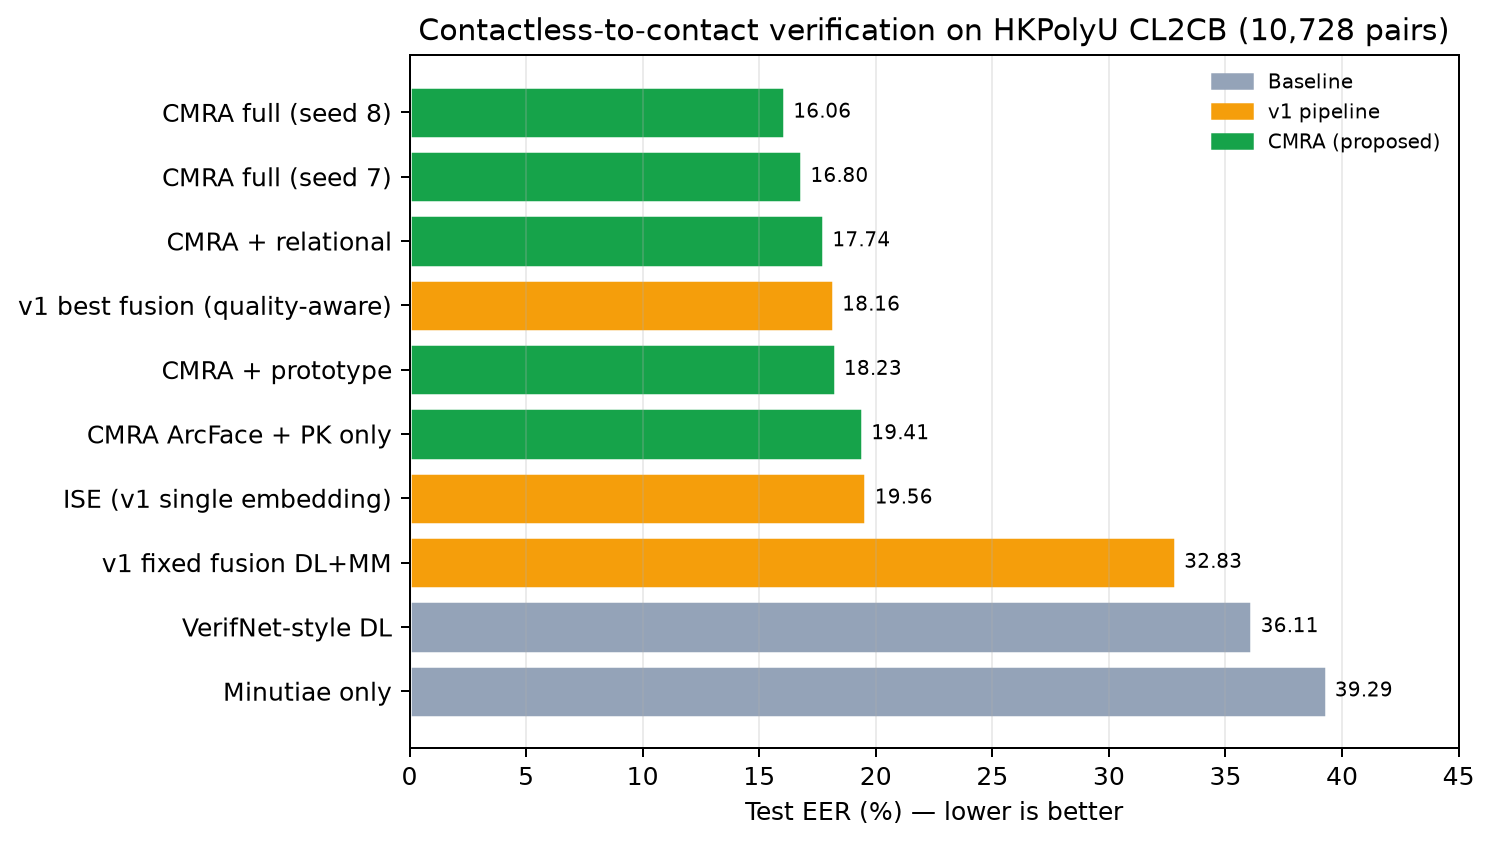
\includegraphics[width=0.78\textwidth]{cmra_comparison.png}
    \caption{Test EER for the baselines, the v1 pipeline and the CMRA ablation on the 10,728-pair test set.}
    \label{fig:comparison}
\end{figure}

\begin{figure}[H]
    \centering
    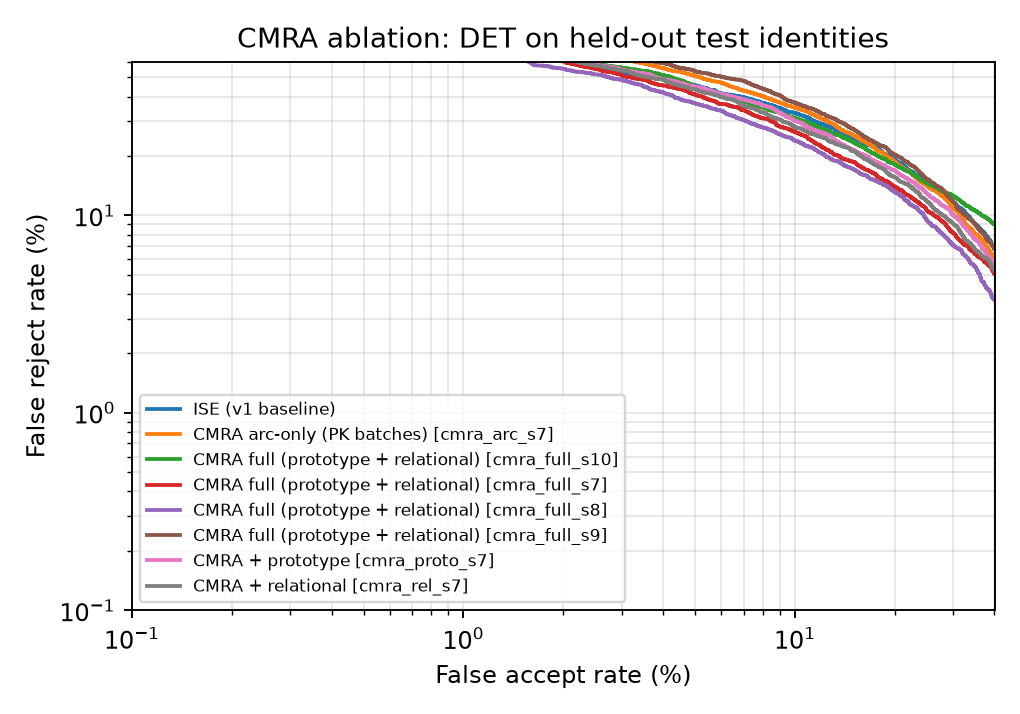
\includegraphics[width=0.7\textwidth]{cmra_det.png}
    \caption{DET curves for the CMRA ablation on held-out test identities (log-log axes).}
    \label{fig:det}
\end{figure}

\subsection{Cross-Session Evaluation}
Table~\ref{tab:cross} reports the supplementary cross-session study on 48 test identities present in both sessions. CMRA seed 8 reaches 14.89\% cross-session EER versus 15.79\% same-session EER on the same identities --- cross-session performance is actually better here, and CMRA beats v1 quality-aware fusion (18.50\% cross-session EER) by 3.6 percentage points. This shows cross-modal relational alignment generalises across sessions, not just within them.

\begin{table}[H]
    \centering
    \caption{Cross-session vs same-session results on 48 test identities (percentages).}
    \label{tab:cross}
    \resizebox{\textwidth}{!}{%
    \begin{tabular}{lcccc}
    \toprule
    Method & Cross-session EER & Cross TAR@1\% & Same-session EER & Same TAR@1\% \\
    \midrule
    CMRA seed 8 (proposed) & 14.89 & 32.81 & 15.79 & 25.64 \\
    v1 quality-aware fusion & 18.50 & 27.66 & 16.26 & 30.35 \\
    ISE (v1 baseline) & 18.89 & 31.57 & 17.43 & 28.36 \\
    Minutiae & 37.66 & 9.90 & 37.72 & 6.86 \\
    \bottomrule
    \end{tabular}%
    }
\end{table}

\subsection{Risk-Controlled Abstention}
Figure~\ref{fig:risk} shows error rate versus coverage for CMRA seed 7, ISE and v1 fusion at a fixed validation threshold. CMRA full reduces error from 16.8\% at 100\% coverage to 5.7\% at 50\% coverage (AURC 0.068 vs 0.084 for ISE), demonstrating that the system can reliably abstain on difficult comparisons. This new capability is absent from the v1 pipeline and from the compared literature.

\begin{figure}[H]
    \centering
    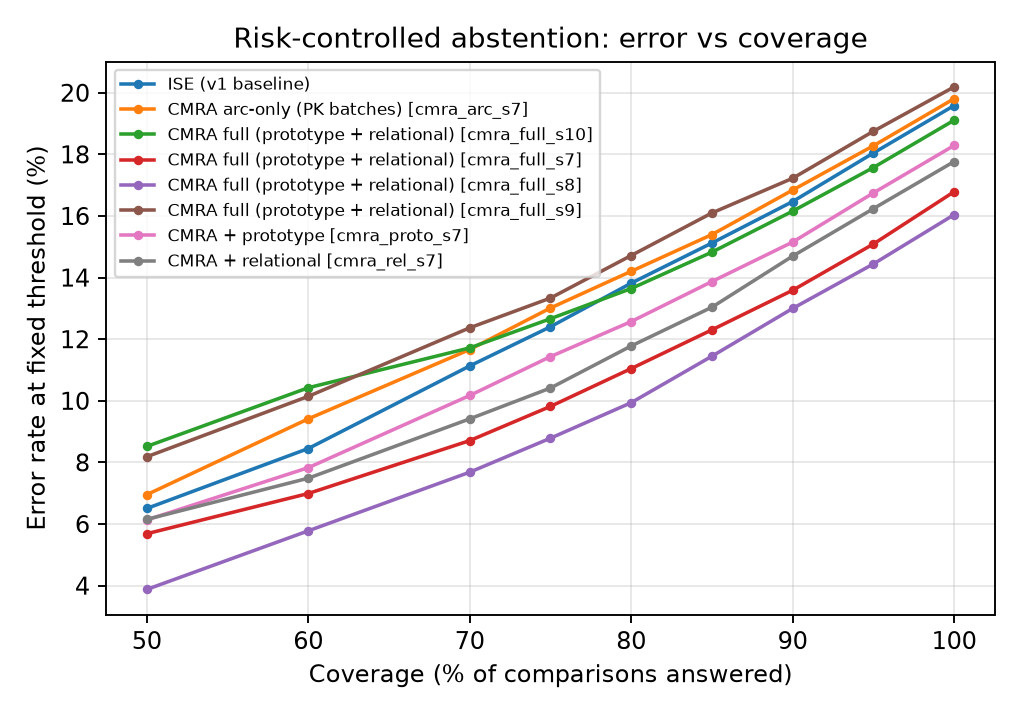
\includegraphics[width=0.7\textwidth]{cmra_risk_coverage.png}
    \caption{Risk--coverage curve: error rate at fixed threshold vs coverage (percentages).}
    \label{fig:risk}
\end{figure}

% ===================== 5. CONCLUSION =====================
\section{Conclusion and Future Work}

This project studied contactless-to-contact fingerprint verification on HKPolyU and proposed Cross-Modal Relational Alignment (CMRA), a single embedding trained to preserve cross-modal relational identity structure using identity-balanced PK batches, ArcFace supervision, prototype consistency and relational consistency losses. CMRA reaches 16.80\% EER and 29.55\% TAR@FAR=1\% on the controlled 10,728-pair test set, beating the reproduced VerifNet-style baseline (36.11\% EER) and its fixed-fusion variant (32.83\% EER) with a simpler pipeline that removes the Siamese branch and score fusion entirely. Risk-controlled abstention further lowers error to 5.7\% at 50\% coverage. Cross-session evaluation on 48 identities confirms generalisation (14.89\% cross-session EER versus 18.50\% for v1 fusion). The work shows that cross-modal relational alignment, not fusion, is the key contribution for lightweight CPU-trainable contactless-to-contact fingerprint verification.

Future work should pursue four directions:
\begin{enumerate}[leftmargin=*]
    \item Learn the minutiae branch jointly with the identity embedding, for example with a minutiae attention network or graph neural network.
    \item Replace hand-crafted quality features with a learned pair-reliability model trained on hard pairs.
    \item Scale training data with identity-consistent synthetic multi-pose generation to close the gap to 2--4\% EER without external real data.
    \item Export the embedding body to OpenVINO and benchmark Intel NPU latency, power and throughput for on-device deployment.
\end{enumerate}

% ===================== REFERENCES =====================
\section*{References}
\addcontentsline{toc}{section}{References}
\begin{enumerate}[leftmargin=*]
    \item G. Parasnis, R. Bhope, A. Chokshi, V. Jain, A. Biswas, D. Kumar, S. Pateriya, V. Anand, V. Kanhangad and V. M. Gadre, ``VerifNet --- A Novel Score Fusion-Based Method Leveraging Wavelets With Deep Learning and Minutiae Matching for Contactless Fingerprint Recognition,'' \emph{IEEE Transactions on Biometrics, Behavior, and Identity Science}, vol. 7, no. 3, Jul. 2025. doi:10.1109/TBIOM.2024.3504281.

    \item S. Pandey, B. Jawade and S. Setlur, ``Ridgeformer: Multi-Stage Contrastive Training for Fine-Grained Cross-Domain Fingerprint Recognition,'' IEEE International Conference on Image Processing (ICIP), 2025. doi:10.1109/ICIP55913.2025.11084677. arXiv:2506.01806.

    \item Z. Pan, X. Guan, J. Feng and J. Zhou, ``Identity-Consistent Multi-Pose Generation of Contactless Fingerprints,'' arXiv:2605.03830, 2026.

    \item S. Peddi, S. Bandyopadhyay and D. Samanta, ``G-MSGINet: A Grouped Multi-Scale Graph-Involution Network for Contactless Fingerprint Recognition,'' arXiv:2505.08233, 2025.

    \item R. Sahoo and A. Namboodiri, ``Fusion2Print: Deep Flash--Non-Flash Fusion for Contactless Fingerprint Matching,'' International Conference on Pattern Recognition (ICPR), 2026. arXiv:2601.02318.

    \item P. Kaplesh, A. Gupta, D. Bansal, S. Sofat and A. Mittal, ``A Systematic Review of End-to-End Framework for Contactless Fingerprint Recognition: Techniques, Challenges, and Future Directions,'' \emph{Engineering Applications of Artificial Intelligence}, 2025. doi:10.1016/j.engappai.2025.110493.

    \item M. Alsmirat, M. M. Khaled and A. A. Sayadi, ``Deep Learning Based Contactless Fingerprint Identification,'' \emph{Cluster Computing}, 2025. doi:10.1007/s10586-025-05829-5.

    \item C. Lin and A. Kumar, ``Matching Contactless and Contact-Based Conventional Fingerprint Images for Biometrics Identification,'' \emph{IEEE Transactions on Image Processing}, vol. 27, no. 4, pp. 2008--2021, 2018.

    \item H. Tan and A. Kumar, ``Minutiae Attention Network with Reciprocal Distance Loss for Contactless to Contact-Based Fingerprint Identification,'' \emph{IEEE Transactions on Information Forensics and Security}, vol. 16, 2021.

    \item J. Deng, J. Guo, N. Xue and S. Zafeiriou, ``ArcFace: Additive Angular Margin Loss for Deep Face Recognition,'' CVPR, 2019.

    \item M. Andreux, T. Angles, J. Exarchakis, R. Leonarduzzi, G. Rochette and L. Thiry, ``Kymatio: Scattering Transforms in Python,'' \emph{Journal of Machine Learning Research}, vol. 21, no. 60, pp. 1--6, 2020.
\end{enumerate}

\end{document}
